\documentclass[a4paper,11pt]{exam}
\printanswers % pour imprimer les réponses (corrigé)
%\noprintanswers % Pour ne pas imprimer les réponses (énoncé)
\addpoints % Pour compter les points
% \noaddpoints % pour ne pas compter les points
%\qformat{\textbf{\thequestion ) } }
\qformat{\textbf{\thequestion )}} % Pour définir le style des questions (facultatif)
\usepackage{color} % définit une nouvelle couleur
\shadedsolutions % définit le style des réponses
% \framedsolutions % définit le style des réponses
\definecolor{SolutionColor}{rgb}{0.8,0.9,1} % bleu ciel
\renewcommand{\solutiontitle}{\noindent\textbf{Solution:}\par\noindent} % Définit le titre des solutions




\makeatletter

\def\maketitle{{\centering%
	\par{\huge\textbf{\@title}}%
	\par{\@date}%
	\par}}


\renewcommand{\thesubsection}{\Alph{subsection}.}   

\makeatother

\lhead{NOM Pr\'enom :}
\rhead{\textbf{Les r\'eponses doivent \^etre justifi\'ees et r\'edig\'ees}}
\cfoot{\thepage / \pageref{LastPage}}


%\usepackage{../../pas-math}
%\usepackage{../../moncours}


%\usepackage{pas-cours}
%-------------------------------------------------------------------------------
%          -Packages nécessaires pour écrire en Français et en UTF8-
%-------------------------------------------------------------------------------
\usepackage[utf8]{inputenc}
\usepackage[frenchb]{babel}
%\usepackage{numprint}
\usepackage[T1]{fontenc}
%\usepackage{lmodern}
\usepackage{textcomp}
\usepackage[french, boxed]{algorithm2e}
\usepackage{hyperref}


%-------------------------------------------------------------------------------

%-------------------------------------------------------------------------------
%                          -Outils de mise en forme-
%-------------------------------------------------------------------------------
\usepackage{hyperref}
\hypersetup{pdfstartview=XYZ}
%\usepackage{enumerate}
\usepackage{graphicx}
\usepackage{multicol}
\usepackage{tabularx}
\usepackage{multirow}
\usepackage{color}
\usepackage{eurosym}


\usepackage{anysize} %%pour pouvoir mettre les marges qu'on veut
%\marginsize{2.5cm}{2.5cm}{2.5cm}{2.5cm}

\usepackage{indentfirst} %%pour que les premier paragraphes soient aussi indentés
\usepackage{verbatim}
\usepackage{enumitem}
\usepackage{booktabs}
\usepackage[usenames,dvipsnames,svgnames,table]{xcolor}

\usepackage{variations}

%-------------------------------------------------------------------------------


%-------------------------------------------------------------------------------
%                  -Nécessaires pour écrire des mathématiques-
%-------------------------------------------------------------------------------
\usepackage{amsfonts}
\usepackage{amssymb}
\usepackage{amsmath}
\usepackage{amsthm}
\usepackage{tikz}
\usepackage{xlop}
\usepackage[output-decimal-marker={,}]{siunitx}
%-------------------------------------------------------------------------------

%-------------------------------------------------------------------------------
%                  -Nécessaires pour écrire des formules chimiquess-
%-------------------------------------------------------------------------------

\usepackage[version=4]{mhchem}

%-------------------------------------------------------------------------------
% Pour pouvoir exploiter les fichiers directement dans beamer
\newcommand{\pause}{\ }
%-------------------------------------------------------------------------------
%                    - Mise en forme avancée
%-------------------------------------------------------------------------------

\usepackage{ifthen}
\usepackage{ifmtarg}


\newcommand{\ifTrue}[2]{\ifthenelse{\equal{#1}{true}}{#2}{$\qquad \qquad$}}

%\newcommand{\kword}[1]{\textcolor{red}{\underline{#1}}}
%-------------------------------------------------------------------------------

%-------------------------------------------------------------------------------
%                     -Mise en forme d'exercices-
%-------------------------------------------------------------------------------
%\newtheoremstyle{exostyle}
%{\topsep}% espace avant
%{\topsep}% espace apres
%{}% Police utilisee par le style de thm
%{}% Indentation (vide = aucune, \parindent = indentation paragraphe)
%{\bfseries}% Police du titre de thm
%{.}% Signe de ponctuation apres le titre du thm
%{ }% Espace apres le titre du thm (\newline = linebreak)
%{\thmname{#1}\thmnumber{ #2}\thmnote{. \normalfont{\textit{#3}}}}% composants du titre du thm : \thmname = nom du thm, \thmnumber = numéro du thm, \thmnote = sous-titre du thm

%\theoremstyle{exostyle}
%\newtheorem{exercice}{Exercice}
%
%\newenvironment{questions}{
%\begin{enumerate}[\hspace{12pt}\bfseries\itshape a.]}{\end{enumerate}
%} %mettre un 1 à la place du a si on veut des numéros au lieu de lettres pour les questions 
%-------------------------------------------------------------------------------

%-------------------------------------------------------------------------------
%                    - Mise en forme de tableaux -
%-------------------------------------------------------------------------------

\renewcommand{\arraystretch}{1.7}

\setlength{\tabcolsep}{1.2cm}

%-------------------------------------------------------------------------------



%-------------------------------------------------------------------------------
%                    - Racourcis d'écriture -
%-------------------------------------------------------------------------------
%Droites
\newcommand{\dte}[1]{$(#1)$}
\newcommand{\fig}[1]{figure $#1$}
\newcommand{\sym}{symétrique}
\newcommand{\syms}{symétriques}
\newcommand{\asym}{axe de symétrie}
\newcommand{\asyms}{axes de symétrie}
\newcommand{\seg}[1]{$[#1]$}
\newcommand{\monAngle}[1]{$\widehat{#1}$}
\newcommand{\bissec}{bissectrice}
\newcommand{\mediat}{médiatrice}
\newcommand{\ddte}[1]{$[#1)$}


% Angles orientés (couples de vecteurs)
\newcommand{\aopp}[2]{(\vec{#1}, \vec{#2})} %Les deuc vecteurs sont positifs
\newcommand{\aopn}[2]{(\vec{#1}, -\vec{#2})} %Le second vecteur est négatif
\newcommand{\aonp}[2]{(-\vec{#1}, \vec{#2})} %Le premier vecteur est négatif
\newcommand{\aonn}[2]{(-\vec{#1}, -\vec{#2})} %Les deux vecteurs sont négatifs

%Ensembles mathématiques
\newcommand{\naturels}{\mathbb{N}} %Nombres naturels
\newcommand{\relatifs}{\mathbb{Z}} %Nombres relatifs
\newcommand{\rationnels}{\mathbb{Q}} %Nombres rationnels
\newcommand{\reels}{\mathbb{R}} %Nombres réels
\newcommand{\complexes}{\mathbb{C}} %Nombres complexes


%Intégration des parenthèses aux cosinus
\newcommand{\cosP}[1]{\cos\left(#1\right)}
\newcommand{\sinP}[1]{\sin\left(#1\right)}


%Probas stats
\newcommand{\stat}{statistique}
\newcommand{\stats}{statistiques}


\newcommand{\homo}{homothétie}
\newcommand{\homos}{homothéties}


\newcommand{\mycoord}[3]{(\textcolor{red}{\num{#1}} ; \textcolor{Green}{\num{#2}} ; \textcolor{blue}{\num{#3}})}
%-------------------------------------------------------------------------------

%-------------------------------------------------------------------------------
%                    - Mise en page -
%-------------------------------------------------------------------------------

\newcommand{\twoCol}[1]{\begin{multicols}{2}#1\end{multicols}}


\setenumerate[1]{font=\bfseries,label=\textit{\alph*})}
\setenumerate[2]{font=\bfseries,label=\arabic*)}


%-------------------------------------------------------------------------------
%                    - Elements cours -
%-------------------------------------------------------------------------------

%Correction d'exercice
\newcommand{\exoSec}[2]{\subsection*{Exercice #1 page #2}}
%-------------------------------------------------------------------------------
%                    - raccourcis d'écriture -
%-------------------------------------------------------------------------------

%Mise en évidence de termes clés
\newcommand{\mykw}[1]{\textcolor{red}{\underline{\textbf{#1}}}}

%Exercices
\newcommand{\exo}[2]{exercice #1 page #2}
\newcommand{\Exo}[2]{Exercice #1 page #2}

\renewcommand{\pause}{\ }

%Intervalles
\newcommand{\interOO}[2]{$]$#1 , #2$[$}
\newcommand{\interOF}[2]{$]$#1 , #2$]$}
\newcommand{\interFO}[2]{$[$#1 , #2$[$}
\newcommand{\interFF}[2]{$[$#1 , #2$]$}



%\usepackage{fullpage}
\author{\ }
\date{7 Octobre 2016}
\title{DS num\'ero 1}


\begin{document}
%	\usepackage{fancyhdr}
%	
%	\pagestyle{fancy}
%	\fancyhf{}
	%\rhead{Share\LaTeX}

	\maketitle
	
\section{Questions à choix multiples}
Pour chaque question, choisir la (ou les) bonne(s) réponse(s).

\begin{questions}
	\question Dans la situation ci-dessous, l'action qui déforme le trampoline est :
	
	\begin{multicols}{2}
	
		\begin{center}
			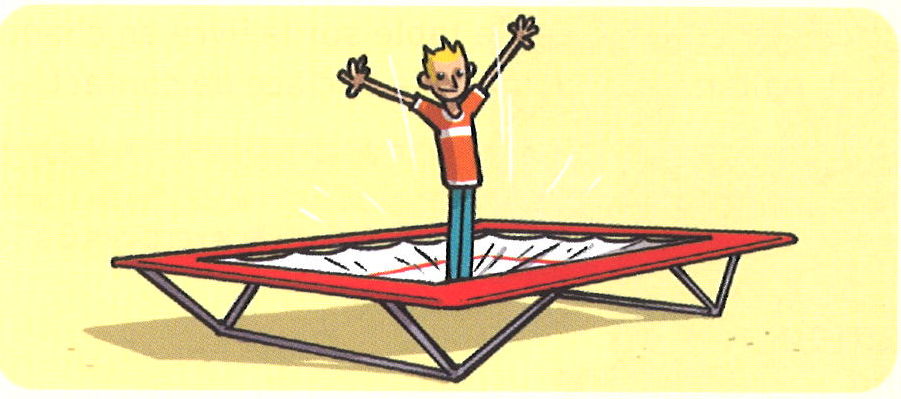
\includegraphics[scale=0.3]{trampo}	
		\end{center}
	
	
		\begin{checkboxes}
			\choice celle exercée par l'enfant sur le trampoline.
			\choice celle exercée par le trampoline sur l'enfant.
			\choice le poids du trampoline.
		\end{checkboxes}
	\end{multicols}
	\question Dans la situation ci-dessous, la force modélisée par la flèche est celle exercée :
	
	\begin{multicols}{2}
		
			
		\begin{center}
			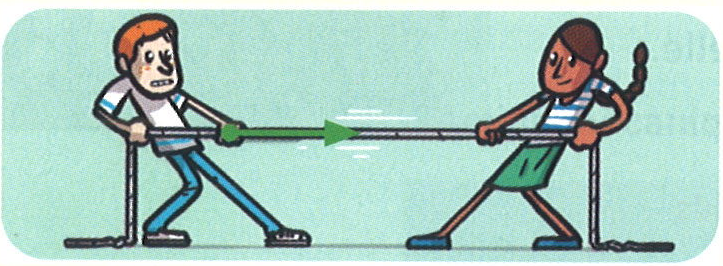
\includegraphics[scale=0.3]{corde}
		\end{center}
		\begin{checkboxes}
			\choice par la fille sur le garçon.
			\choice par la corde sur le garçon.
			\choice par la fille sur la corde.
		\end{checkboxes}
		
	\end{multicols}

	\question Dans la situation ci-dessous, le plongeur est soumis :
	
	\begin{multicols}{2}
		
		
		\begin{center}
			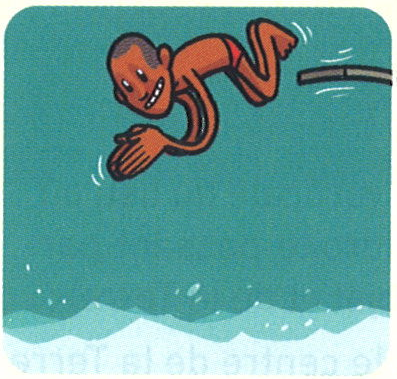
\includegraphics[scale=0.3]{plong}
		\end{center}
		\begin{checkboxes}
			\choice à l'action exercée par le plongeoir.
			\choice à l'action exercée par la Terre.
			\choice à l'action exercée par l'air.
		\end{checkboxes}
	\end{multicols}

\end{questions}


\section{Diagramme objet-interaction}

Pour chaque diagramme objet-interaction, déterminer quelle est la situation décrite.

\begin{multicols}{2}
	\begin{questions}
		\question	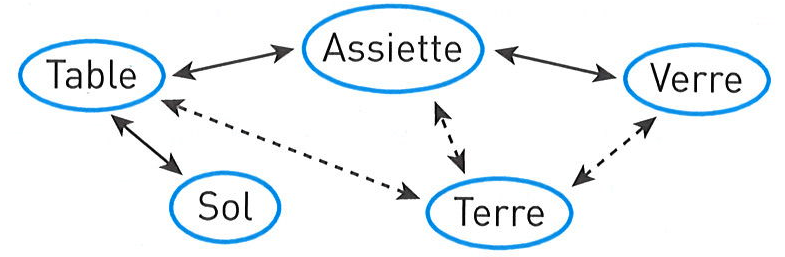
\includegraphics[scale=0.35]{doi1}
		
		\question 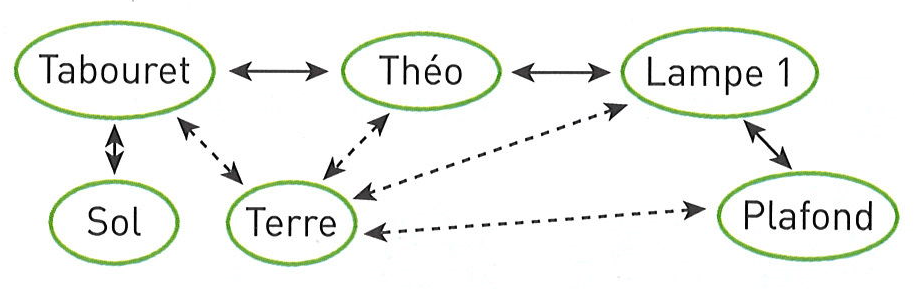
\includegraphics[scale=0.35]{doi2}
		
	\end{questions}
\end{multicols}


\section{Des actions qui se compensent}

Un corps est soumis à des forces qui se compensent.

\begin{questions}
	\question Dans quels cas des forces se compensent-elles ?
	\question Ce corps est au repos :
	
	\begin{parts}
		\part Son état de repos va-t-il être modifié ?
		\part Que faut-il pour que l'état soit modifié ?
	\end{parts}
	
\end{questions}

\section{Un coup de marteau}

Giselle pose du plancher. Elle cherche à comprendre ce que subit le clou lorsqu'on vient le frapper avec le marteau.

\begin{questions}
	\question \'Etablir un diagramme objet-interaction pour l'objet <<clou>>.
	\question Faire un schéma de la situation et représenter les forces qui s'exercent sur le clou.
	\question Quel est l'effet de l'ensemble des actions qui s'exercent sur le clou.
	
\end{questions}

\subsection*{Données}
	\begin{itemize}
		\item Force exercée par le marteau sur le clou : \num{50000} N;
		\item Force exercée par la planche sur le clou : \num{5000} N;
		\item \'Echelle : 1 cm $\leftrightarrow$ \num{10000} N.
	\end{itemize}

\section{Grues de chantier}

Les grues permettent de déplacer de lourdes charges sur un chantier. On s'intéresse à la charge soulevée par la grue.

\begin{questions}
	\question Avec quels objets la charge est-elle en interaction ? Préciser à chaque fois le type d'interaction.
	\question Ètablir le diagramme objet-interaction de la charge.
	\question Représenter sur un schéma la force de \num{10000} N exercée par le câble de la grue sur la charge. Préciser l'échelle choisie.
\end{questions}


\newpage 

\section{Caractéristiques d'une force}

Dans chacun de ces 6 cas donner les caractéristiques de la force représentée (direction, sens et point d'application).

\begin{center}
%\begin{multicols}{2}
	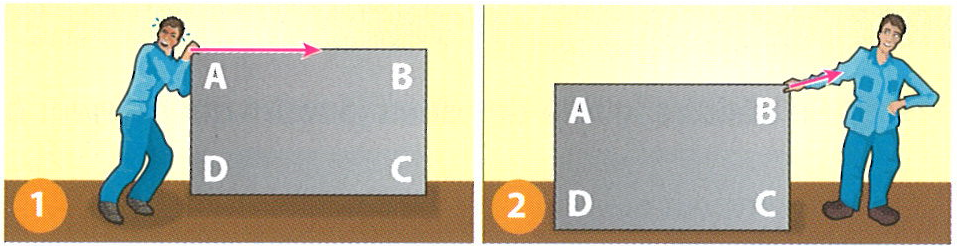
\includegraphics[scale=0.5]{forces_1}
	
	\vspace*{0.5cm}
	
	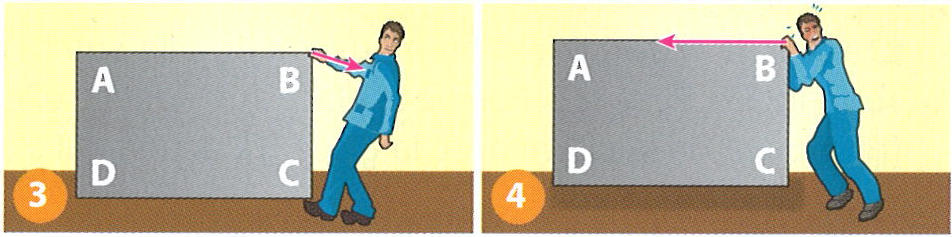
\includegraphics[scale=0.5]{forces_2}
%\end{multicols}

	\vspace*{0.5cm}
	
	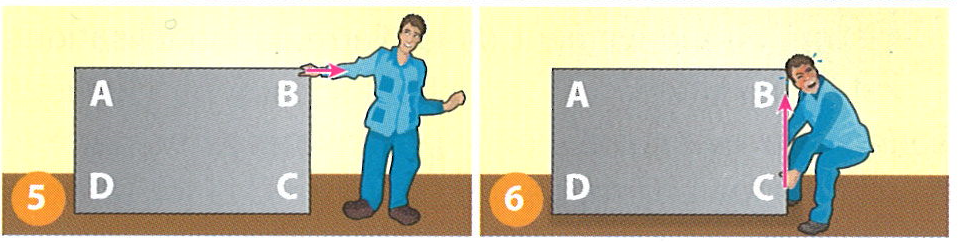
\includegraphics[scale=0.5]{forces3}
\end{center}


\label{LastPage}

\end{document}